% ---------------------------------------------------------------------
% EG author guidelines plus sample file for EG publication using LaTeX2e input
% D.Fellner, v2.02, Jan 25, 2017


\title[DynAIRx]%
      {Patient History Visualization for Structured Medication Reviews: a design study}

% for anonymous conference submission please enter your SUBMISSION ID
% instead of the author's name (and leave the affiliation blank) !!
% for final version: please provide your *own* ORCID in the brackets following \orcid; see https://orcid.org/ for more details.
\author[L. Hama \& R.A. Ruddle \& others]{
\parbox{\textwidth}{
\centering 
L. Hama$^{10}$\orcid{0000-0003-1912-4890}, R.A. Ruddle$^{10}$\orcid{0000-0001-8662-8103}, A.S. Abuzour$^{1,2}$, M. Abaho$^{3}$, A. Aslam$^{2,8}$, D. Bollegala$^{3}$, H. Cant$^{6}$, A. Clegg$^{1,2}$, M. Gabbay$^{3}$, A. Griffiths$^{7}$, F. Jury$^{6}$, G. Leeming$^{3}$, E. Lo$^{3}$, F.S. Mair$^{5}$, S. Maskell$^{3}$, E. McCloskey$^{3}$, M. O’Connell$^{6}$, P. Schofield$^{11}$, O. Popoola$^{9}$, S. Relton$^{2,8}$, E. Shantsila$^{3}$, M. Sperrin$^{6}$, T. Van Staa$^{6}$, S.A. Wilson$^{3}$, A.A. Woodall$^{3,4}$, I. Buchan$^{3}$, L.E. Walker$^{3}$
}
\\
{\parbox{\textwidth}{
\centering 
$^{1}$Academic Unit for Ageing \& Stroke Research, University of Leeds, Bradford Teaching Hospitals NHS Foundation Trust, Bradford, UK \\
$^{2}$Faculty of Medicine and Health, School of Medicine, University of Leeds, Leeds, UK \\
$^{3}$Wolfson Centre for Personalised Medicine, University of Liverpool, Liverpool, UK \\
$^{4}$Directorate of Mental Health and Learning Disabilities, Powys Teaching Health Board, Bronllys, UK \\
$^{5}$General Practice and Primary Care, School of Health and Wellbeing, University of Glasgow, Glasgow, UK \\
$^{6}$Division of Informatics, Imaging \& Data Science, University of Manchester, Manchester, UK \\
$^{7}$Public Advisor, NIHR Applied Research Collaboration NorthWest Coast \\
$^{8}$Leeds Institute for Data Analytics, University of Leeds, Leeds, UK \\
$^{9}$Merseycare NHS Foundation Trust, Liverpool, UK \\
$^{10}$School of Computing, University of Leeds, Leeds, UK \\
$^{11}$Institute of Population Health, University of Liverpool, Liverpool, UK
}
}
}


\usepackage{amsmath}
\usepackage{amssymb}
\usepackage{amsthm}
\usepackage{tabularx}
\usepackage{hhline}
% plotting
\usepackage{pgfplots}
\usepackage{booktabs}
\usepackage{multirow}
 
\DeclareMathOperator{\True}{True}
\DeclareMathOperator{\False}{False}
\DeclareMathOperator{\members}{members}
\DeclareMathOperator{\intersectionId}{intersectionId}
\DeclareMathOperator{\intersectionMembers}{intersectionMembers}
\DeclareMathOperator{\ElementIndex}{ElementIndex}
\DeclareMathOperator{\IntersectionIndex}{IntersectionIndex}


% ------------------------------------------------------------------------

% if the Editors-in-Chief have given you the data, you may uncomment
% the following five lines and insert it here
%
% \volume{36}   % the volume in which the issue will be published;
% \issue{1}     % the issue number of the publication
% \pStartPage{1}      % set starting page


%-------------------------------------------------------------------------
\begin{document}

% uncomment for using teaser
% \teaser{
%  \includegraphics[width=\linewidth]{eg_new}
%  \centering
%   \caption{New EG Logo}
% \label{fig:teaser}
%}

\maketitle
%-------------------------------------------------------------------------
\begin{abstract}

This design study focuses on generating and validating chart based design choices as visual summaries for patient history records to be used whilst conducting Structured Medication Reviews (SMR) by general practitioners and pharmacists. The design study follows a well known methodology to characterise the domain problem, generate design choices and evaluate them with eight domain experts and 11 non-domain experts. Mock SMRs were conducted with domain experts in order to understand the domain problem (SMRs) and generate data abstraction in order to conduct the design study work. The results of the design study shows that out of 14 unique chart types 11 of them are deemed suitable by domain experts to be used to visualise patient records. The contributions of this work are: conducting mock SMRs, problem characterisation, design space exploration and evaluation, and our reflections.

%-------------------------------------------------------------------------
%  ACM CCS 1998
%  (see http://www.acm.org/about/class/1998)
% \begin{classification} % according to http:http://www.acm.org/about/class/1998
% \CCScat{Computer Graphics}{I.3.3}{Picture/Image Generation}{Line and curve generation}
% \end{classification}
%-------------------------------------------------------------------------
%  ACM CCS 2012
%   (see http://www.acm.org/about/class/class/2012)
%The tool at \url{http://dl.acm.org/ccs.cfm} can be used to generate
% CCS codes.
%Example:
\begin{CCSXML}
<ccs2012>
<concept>
<concept_id>10003120.10003145.10003151</concept_id>
<concept_desc>Human-centered computing~Visualization systems and tools</concept_desc>
<concept_significance>500</concept_significance>
</concept>
<concept>
<concept_id>10003120.10003145.10011769</concept_id>
<concept_desc>Human-centered computing~Empirical studies in visualization</concept_desc>
<concept_significance>500</concept_significance>
</concept>
<concept
<concept_id>10010405.10010444</concept_id>
<concept_desc>Applied computing~Life and medical sciences</concept_desc>
<concept_significance>500</concept_significance>
</concept>
<concept>
<concept_id>10010405.10010476</concept_id>
<concept_desc>Applied computing~Computers in other domains</concept_desc>
<concept_significance>500</concept_significance>
</concept>
</ccs2012>
\end{CCSXML}

\ccsdesc[500]{Human-centered computing~Visualization systems and tools}
\ccsdesc[500]{Human-centered computing~Empirical studies in visualization}
\ccsdesc[500]{Applied computing~Life and medical sciences}
\ccsdesc[500]{Applied computing~Computers in other domains}


\printccsdesc   
\end{abstract}  
%-------------------------------------------------------------------------
\section{Introduction}
General practitioners (GPs) and pharmacists conduct Structured Medication Reviews (SMRs) \cite{madden2022early} as "a comprehensive and clinical review of a patient’s medicines and detailed aspects of their health" \cite{nhs2021}. SMRs involve consultation with patients, considering their medical history (diagnoses, symptoms, current medication, investigations, etc.) ~\cite{madden2022early}.
In the UK medical history is accessed via an electronic health record (EHR) system such as EMIS \cite{emishealth2023}. Such systems provide detailed information about a patient’s medical history but information that is needed to conduct SMRs in complex patients is not presented in a manner that is time efficient.

A wide variety of techniques have been applied to visualise EHRs of individual patients and cohorts of patients in previous research~\cite{wang2022ehr,dowding2015dashboards}, but not for the purpose of conducting medication reviews. The present work follows a design study methodology~\cite{sedlmair2012design} to select candidate charts for visual histories of patient records for SMRs. 
Then, four mock patient SMRs were carried out to establish user requirements in terms of: (a) questions that GPs and or pharmacists typically want to answer in an SMR, and (b) the attributes of medical histories that are required.
A design space was determined by mapping the attributes to the data types that different types of visualization support.
Low-fidelity (paper and pencil) prototypes were used to evaluate the design choices and produce a shortlist of visualizations for groups of SMR questions.

This paper makes three contributions based on the methodology \cite{sedlmair2012design} followed.
First, problem characterisation, that is, analysing and data abstraction using mock SMRs.
Second, it presents candidate visualizations for six combinations of data types. Third, a Python package that implements the outcomes \cite{dynairxvis}.

The rest of this work is structured as follows: It starts with an extensive background review of techniques (charts) used to visualise EHR. Then it summarises the work done to understand the nature of SMRs using the four mock SMRs. Section \ref{sec:design} then describes the design space exploration approach and the outcomes and one round of validation of our design choices. The last section outlines the implementation of the design study.

% relatedwork2

\section{Related Work}\label{sec:relatedwork}
\begin{table*}[!p]
\centering
\caption{The table summarises visualization techniques, domains, measurements and data types used in EHR dashboards. Abbreviations: BP=Blood Pressure, QI=Quality Improvement, N=Nominal, Q=Quantitative, O=Ordinal, and T=Temporal}
\begin{tabularx}{\textwidth}{|>{\raggedright\arraybackslash}m{1.7cm}|>{\raggedright\arraybackslash}m{3.1cm}|>{\raggedright\arraybackslash}m{3.1cm}|>
{\raggedright\arraybackslash}m{1.1cm}|X|}
% {\raggedright\arraybackslash}m{1.1cm}|m{2.5cm}|}
% {|m{2cm}|X|X|m{1cm}|m{2.5cm}|}
\hhline{-----}\toprule
 \textbf{Chart type} & \textbf{Domains} & \textbf{Measurements} & \textbf{Data type(s)} & \textbf{Reviewed publication(s)} \\ \hline
% \midrule
Bar & Stroke cohort, Pain management, Diabetes, Anaesthesia, Antibiotic prescribing QI, Diabetes Hospital Admissions, QI & Length of Stay (LOS), Patient counts, Pain score, Various (blood, lungs etc), Odds, Minutes, Statistics, Categorical counts & N, Q, T & \vspace{-4em} \cite{daley2013clinical}, \cite{elshehaly2020qualdash}, \cite{hester2019timely}, \cite{loorak2015timespan}, \cite{laurent2021development}, \cite{opie2021requirements},  \cite{stone2019dashboard}, \cite{wong2020dashboard}, \cite{linder2010} \\ \hline
Box & Diabetes & Odds & Q & \cite{wong2020dashboard} \\ \hline
Bar graph (bar meter) & Inter-operative Care & Various (Vital Signs, Glucose, Oxygen level etc) & Q & \cite{kheterpal2018impact} \\ \hline
Gauge & Mental Health, Diabetes & Lipid, Renal function, Blood glucose, Other & Q & \cite{daley2013clinical}, \cite{yandrapalli2019development}  \\ \hline
Glyph & Not known & Test levels (low to high) & N & \cite{linhares2022clinicalpath} \\ \hline
Icon & Diabetes, ICU monitoring, QI record improvement & Status, Trend (up/down), Yes/No & Q, N & \cite{calzoni2020graphical}, \cite{koopman2011diabetes}, \cite{mcmenamin2011patient} \\ \hline
Line & Hypertension, Stroke cohort & BP, Event instances, Minutes, Diagnostics, Categorical, Blood tests, Statistics & N, Q, T & \vspace{-2em}  \cite{fadel2021visual}, \cite{elshehaly2020qualdash},
\cite{hester2019timely}, \cite{linhares2022clinicalpath}, \cite{loorak2015timespan}, \cite{opie2021requirements}, \cite{stone2019dashboard}, \cite{yandrapalli2019development} \\ \hline
List & Elderly Care, Inter-operative, Stroke cohort, Diabetes & Diagnostics, Incident tracking, Dosage & N, Q, Text & \vspace{-2em} \cite{daley2013clinical}, \cite{kheterpal2018impact}, \cite{koopman2011diabetes}, \cite{loorak2015timespan} \\ \hline
Organs & Inter-operative Care & Status (Green, Amber, Red) & N & \cite{kheterpal2018impact} \\ \hline
Parallel Coordinates & General Practice & Multivariate & Q & \cite{de2015design} \\ \hline
Pie & Elderly Care, QI & Observation Levels, Counts & N, Q & \cite{daley2013clinical}, \cite{elshehaly2020qualdash} \\ \hline
Sankey & Stroke cohort, Pain management & Patient counts, Pain categories, Months & N, Q, T & \cite{loorak2015timespan}, \cite{opie2021requirements} \\ \hline
Signal Element & Generic Surveillance & Miscellaneous & Q & \cite{kraus2018using} \\ \hline
Scatter & Post Anaesthesia, ICU monitoring & Various (Vital Signs, Glucose, Oxygen levels etc), Length of Stay (LOS) & N, Q & \vspace{-2em} \cite{calzoni2020graphical}, \cite{schulz2020case} \\ \hline
Table & Ventilator Management ICU, Pain management, Diabetes, Mental Health, BP control, Diabetes Hospital Admissions, Adverse Drug Events, Radiology, QI & Drug, Date/Interval, Event, Date, Yes/No, Length of Stay (LOS), Patient demographics, Events (admissions), Range of days, Patient counts, BP & Q, O, T, N, Text & \vspace{-5em}\cite{daley2013clinical}, \cite{hester2019timely}, \cite{mcmenamin2011patient}, \cite{wong2020dashboard}, \cite{morgan2008radiology}, \cite{koopman2011diabetes}, \cite{laurent2021development}, \cite{stone2019dashboard}, \cite{zaydfudim2009implementation}, \cite{opie2021requirements}, \cite{stinson2012health}, \cite{stone2019dashboard}  \\ \hline
% ahern et al == stinson2012health
Traffic lights & Diabetes, BP control, Radiology & Status, BP, Test status (due, done etc) & O, N & \cite{stinson2012health}, \cite{morgan2008radiology}, \cite{koopman2011diabetes} \\ \hline
% UI buttons & Interoperative Care & Status (Green, Amber, Red) & N & \cite{kheterpal2018impact} \\ \hline
% \hline

\end{tabularx}
\label{table:dashboards}
\end{table*}

% \begin{table*}[!h]
\centering
\caption{Visualization techniques used in EHR dashboards, with one example domain, measurement, and publication per chart type. Data types (N=Nominal, Q=Quantitative, O=Ordinal, T=Temporal) reflect their usage as reported in the reviewed publications.}
\begin{tabularx}{\textwidth}{|>{\raggedright\arraybackslash}m{2.2cm}|>{\raggedright\arraybackslash}m{3.2cm}|>{\raggedright\arraybackslash}m{3.3cm}|>{\raggedright\arraybackslash}m{1.3cm}|X|}
\hhline{-----}\toprule
 \textbf{Chart type} & \textbf{Example domain} & \textbf{Example measurement} & \textbf{Data type(s)} & \textbf{Publication} \\ \hline
Bar & Stroke cohort & Length of Stay (LOS) & N, Q, T & \cite{daley2013clinical} \\ \hline
Box & Diabetes & Odds & Q & \cite{wong2020dashboard} \\ \hline
Bar meter & Inter-operative Care & Vital signs & Q & \cite{kheterpal2018impact} \\ \hline
Gauge & Mental Health & Blood glucose & Q & \cite{yandrapalli2019development} \\ \hline
Glyph & -- & Test levels & N & \cite{linhares2022clinicalpath} \\ \hline
Icon & Diabetes & Trend (up/down) & Q, N & \cite{calzoni2020graphical} \\ \hline
Line & Hypertension & Blood pressure (BP) & N, Q, T & \cite{fadel2021visual} \\ \hline
List & Elderly care & Dosage & N, Q, Text & \cite{koopman2011diabetes} \\ \hline
Organs & Inter-operative Care & Status (Green/Amber/Red) & N & \cite{kheterpal2018impact} \\ \hline
Parallel Coordinates & General practice & Multivariate & Q & \cite{de2015design} \\ \hline
Pie & Quality Improvement & Observation levels & N, Q & \cite{elshehaly2020qualdash} \\ \hline
Sankey & Pain management & Pain categories & N, Q, T & \cite{opie2021requirements} \\ \hline
Signal element & Surveillance & Miscellaneous & Q & \cite{kraus2018using} \\ \hline
Scatter & ICU monitoring & Oxygen levels & N, Q & \cite{schulz2020case} \\ \hline
Table & Diabetes & Patient demographics & Q, O, T, N, Text & \cite{stone2019dashboard} \\ \hline
Traffic lights & BP control & Test status (due/done) & O, N & \cite{morgan2008radiology} \\ \hline
\end{tabularx}
\label{table:dashboards}
\end{table*}


The present work aims to develop visual summaries of patient medical histories in the context of SMR. Expert input from clinicians who are part of the project team and focus groups with other clinicians shows that these summaries need to contain longitudinal information on the conditions, medications, and investigations of a patient.

From the focus group work \cite{abuzour2023dynairx}, the DynAIRx project team has identified items called a wish list that stress the need for a timeline to present visual summaries of the combined patient record. The focus group participants have identified the need to visualise changes over time and prescription timelines, among others.

Visual summaries also need to present the information in a much easier to digest form than the multiple tabs and click-heavy user interfaces of general-purpose EHR systems \cite{abuzour2023dynairx}. 
% The main finding to the best of our knowledge is that there is no work that is closely related to the present work.
To our knowledge, there has been no previous research on how to visualise patient histories specifically for SMRs.
However, a considerable body of work has investigated dashboards for EHRs~\cite{dowding2015dashboards} and EHR visualization techniques~\cite{wang2022ehr}.
We approached the related work using a semi-systematic method \cite{snyder2019literature}, combining two review papers with forward citation tracking. The first was a review by Dowding et al. \cite{dowding2015dashboards} and the second was a state-of-the-art review by Wang and Laramee \cite{wang2022ehr}. The criteria used to select the publications from these sources were: the work uses patient-level or cohort EHR, and is developed for clinical use.

\begin{table*}[!h]
\centering
 % from the Wang and Laramee review \cite{wang2022ehr} (Table 19 in their work). In the Wang and Laramee review bar, line and pie charts are grouped as "standard 2D".
\caption{The table shows the list of visualization techniques used in publications matching our criteria and aims. It also shows measurements visualised in the context of the present work (condition, medication, investigation) and the datatype of the measurements. Abbreviations: C=Condition, M=Medication, I=Investigation (tests or observations), N=Nominal, Q=Quantitative, O=Ordinal, and T=Temporal}
\begin{tabularx}
{\textwidth}{|m{1.7cm}|m{2cm}|X|m{1.1cm}|X|}
\hhline{-----}
\toprule
 \textbf{Chart type} & \textbf{Condition, Medication, Investigation} & \textbf{Measurement(s)} & \textbf{Data type(s)} & \textbf{Reviewed publication(s)} \\ \hline
% \midrule
Bar, Pie, Line & C, I & Dates, States (biological, treatment), Blood tests  & N, Q, T, O & \cite{bernard2015visual}, \cite{bernard2018using}, \cite{kwon2020dpvis}, \cite{zhang2018idmvis} \\ \hline
% Beeswarm & C, M, I & Visit, State and Age & Q, N & \cite{kwon2020dpvis} \\ \hline
Box & I & Prostate-Specific Antigen, Insulin and carbohydrates & Q & \cite{bernard2018using}, \cite{jin2020carepre}. \cite{zhang2018idmvis} \\ \hline
Bubble & C, M, I & Events \& duration & T, N & \cite{kamaleswaran2016physioex} \\ \hline
Chord & C, M, I & State transition (weighted),  & N & \cite{kwon2020dpvis}, \cite{alemzadeh2020visual} \\ \hline
Glyph & C, M, I & State transition, Organs/abnormality, Events, Patient state (diagnosis, treatment, visits) & N & \cite{gotz2014decisionflow}, \cite{kwon2020dpvis}, \cite{jin2020carepre}, \cite{guo2017eventthread}, \cite{zhang2018idmvis} \\ \hline
Histogram & M, I & Medication, Status Counts & Q & \cite{bernard2018using}, \cite{kwon2018retainvis} \\ \hline
Heatmap & C, M, I & Event relationship, Physio data (heart rate, oxygen flu) & N, Q, T & \cite{bernard2018using}, \cite{kamaleswaran2016physioex}, \cite{wang2021lettervis}, \cite{loorak2015timespan} \\ \hline
Parallel Coordinates & I & BMI, Glucose Level & Q & \cite{alemzadeh2020visual} \\ \hline
Parallel sets & C, M, I & Event relationship, State transition (weighted) & T, N & \cite{gotz2014decisionflow}, \cite{kwon2020dpvis}, \cite{jin2020carepre} \\ \hline
Sankey & C, M, I & Event sequence progression, Events & T, N & \cite{gotz2014decisionflow}, \cite{wongsuphasawat2011outflow} \\ \hline
Scatter & M, I & Missing data, Dosage, Date, Phone, Sex & N & \cite{alemzadeh2020visual}, \cite{wang2021lettervis} \\ \hline
Stream graph & C, M, I & Events (classification) \& duration, Time (seroconversion) & T, N & \cite{kamaleswaran2016physioex}, \cite{kwon2020dpvis} \\ \hline
% Timeline & C, M, I & Event & T, N & \cite{guo2017eventthread} \\ \hline
Treemap & C, M, I & Event freequency & Q, N & \cite{guo2018visual}, \cite{guo2017eventthread} \\ \hline

\end{tabularx}

\label{table:ehr-star}
\end{table*}
% \begin{table*}[!h]
\centering
\caption{Visualization techniques used in publications matching our criteria and aims. For each chart type, one example domain (condition, medication, or investigation), one measurement, and one publication are listed. Data types (N=Nominal, Q=Quantitative, O=Ordinal, T=Temporal) are as reported in the reviewed studies.}
\begin{tabularx}{\textwidth}{|m{2.0cm}|m{2.0cm}|X|m{1.1cm}|X|}
\hhline{-----}\toprule
 \textbf{Chart type} & \textbf{C / M / I} & \textbf{Example measurement} & \textbf{Data type(s)} & \textbf{Publication} \\ \hline
Bar / Pie / Line & Condition & Blood tests & N, Q, T, O & \cite{bernard2015visual} \\ \hline
Box & Investigation & Prostate-Specific Antigen & Q & \cite{jin2020carepre} \\ \hline
Bubble & Medication & Event duration & T, N & \cite{kamaleswaran2016physioex} \\ \hline
Chord & Condition & State transitions & N & \cite{alemzadeh2020visual} \\ \hline
Glyph & Investigation & Patient state (diagnosis/treatment) & N & \cite{gotz2014decisionflow} \\ \hline
Histogram & Medication & Medication counts & Q & \cite{kwon2018retainvis} \\ \hline
Heatmap & Investigation & Physiological data (heart rate) & N, Q, T & \cite{wang2021lettervis} \\ \hline
Parallel Coordinates & Investigation & Glucose level & Q & \cite{alemzadeh2020visual} \\ \hline
Parallel Sets & Condition & State transitions & T, N & \cite{jin2020carepre} \\ \hline
Sankey & Condition & Event progression & T, N & \cite{wongsuphasawat2011outflow} \\ \hline
Scatter & Investigation & Dosage vs. outcome & N & \cite{alemzadeh2020visual} \\ \hline
Stream graph & Condition & Time progression (seroconversion) & T, N & \cite{kwon2020dpvis} \\ \hline
Treemap & Condition & Event frequency & Q, N & \cite{guo2018visual} \\ \hline
\end{tabularx}
\label{table:ehr-star}
\end{table*}


\subsection{EHR Dashboards}\label{section:ehr-dashboards}

% Dashboards are used for "data-driven decision making" \cite{sarikaya2018we} and are increasingly integrated into various software applications, first appearing in the 1990s as "a graphical summary of various types of information" \cite{cahyadi2016beyond}. Dashboards in clinical care are subject to various health informatics research, including some design recommendations \cite{brown2016interface} in the context of audit and feedback dashboards, such as the use of line graphs to show trends including relevant nonclinical data \cite{brown2016interface}.

%rar% The second aim of this review was to review dashboards and visualizations in wider healthcare environments.
Table \ref{table:dashboards} lists the publications, visualization techniques that appear in them, the healthcare domain, the healthcare record measurements for which the techniques were used, and the datatypes of those measurements.
The first observation from the publications in Table \ref{table:dashboards} is that the technique appearing the most is the use of tables along with bar and line charts. Some dashboards combine tables with other visualization techniques such as bars, pie, and traffic light colours \cite{koopman2011diabetes,stinson2012health,daley2013clinical}.

The second observation is that we can see some uncommon visualization techniques in Table \ref{table:dashboards}. For example, the use of what is called a "signal element" \cite{schulz2020case} is designed to create dashboards using the Arden syntax\cite{hripcsak1994writing} which is a markup language for sharing medical language. An important concept in EHR data is a threshold or a range of thresholds for particular measurements. This explains the appearance of a "bar graph (bar meter)" in the chart-type column of Table \ref{table:dashboards}.

The third observation is the variety of health record measurements appearing in the various dashboards listed in Table \ref{table:dashboards}. Unsurprisingly, there are time (date/interval, range of days or duration), state, trend, events, and in many cases combinations of such measurements. Visualization of status could be of a test being tracked (due, done, etc.) \cite{stinson2012health}, or the status of an organ \cite{kheterpal2018impact,calzoni2020graphical}.

The fourth observation is about rare techniques such as glyphs for patient visits (as noted by Wang and Laramee \cite{wang2022ehr}). One of the dashboards \cite{kheterpal2018impact} uses an outline of the human upper body organs as the main view of their dashboard with bar graphs of measurements such as temperature and various blood test measurements. A single icon traffic light combined with text values for various measurements is also used to indicate status \cite{kraus2018using}. Another visualization technique in the context of the Intensive Care Unit (ICU) monitoring dashboard is the use of icons to represent the trend of a particular measurement over time \cite{calzoni2020graphical}. The technique used is a single-value scatter plot that represents the measurement in both its state (normal/abnormal) and its quantity but also where the measurement lies within the ranges of clinical guidelines over time. Such visualization would mean that even if multiple measurements cannot be combined in a single plot, there could be multiple plots in a more compact and "readable" summary visualization.

\subsection{EHR Visualization Techniques}\label{section:ehr-techniques}

The techniques listed in Table \ref{table:ehr-star} are those that appeared in a publication that matched the criteria for the present work. The second column of Table \ref{table:ehr-star} lists the categories (conditions, medications, and investigations). % This study uses the same three categories in the mock SMRs (see Section \ref{sec:understanding-smrs}).

Finally, looking through Table \ref{table:dashboards} and Table \ref{table:ehr-star}, the chart types that appear in both are bar, line, scatter, box (box-and-whisker), glyph-based displays, parallel coordinates, and Sankey diagrams. This is expected from the reviewed dashboards in the case of Table \ref{table:dashboards}, but the Wang and Laramee review focuses on the wider area of visualising EHR data. Tables as a visualization technique in the case of dashboards are not considered or do not appear in Wang and Laramee's review \cite{wang2022ehr}.

% \subsection{Summary}\label{sec:related-work-summary}

% Analysis of the existing literature revealed a diverse array of chart types that are used for the presentation of patient-level and cohort data, laying a foundational understanding necessary before any design space exploration is carried out. This review is followed by a close understanding of the domain problem (SMRs), which will be discussed next as part of the "discover" stage of the methodology.


% 
\begin{table*}
\centering
\begin{tabularx}{\textwidth}{|X|X|X|X|X|}
\hhline{|=====|}
\multicolumn{1}{|c|}{\textbf{Data source}} & \multicolumn{4}{c|}{\textbf{Data type}} \\ \hline 
\multicolumn{1}{|c|}{} & \multicolumn{1}{c|}{\textbf{Categorical}} & \multicolumn{1}{c|}{\textbf{Numeric}} & \multicolumn{1}{c|}{\textbf{Text}} & \multicolumn{1}{c|}{\textbf{Date/Time}} \\ \hline
\textbf{Multimorbidity} & Diseases/Conditions & Severity & & Diagnosis Date \\ \hline
\textbf{Medication List} & Drug Name & Dosage & Frequency & Prescription Date \\ \hline
\textbf{Vital Signs} & Blood Pressure, Heart Rate, Respiratory Rate, Temperature & Levels/Readings & Measurement Date & \\ \hline
\textbf{Laboratory Results}& Test Name & Test Results & Radiologist's Report& Test Date \\ \hline
\textbf{Medical History}& Allergies/Reactions & & Past Medical Events, Surgeries, Hospitalizations & Event Date\\ \hline
\textbf{Social History}& Lifestyle Factors&& Occupation, Living Conditions & Lifestyle Change Date \\ \hline
\textbf{Family History} & Medical Conditions && Family Medical Conditions & Condition Onset Date \\ \hline
\textbf{Patient-reported Outcomes} & Symptoms && Patient Concerns & Report Date \\ \hline
\textbf{Clinical Guidelines}& Conditions & & Description/Details & Publication Date \\ \hline
% Medication Adherence & Adherence Level & Pill Count & Pharmacy Records& Last Medication Pickup Date\\ \hline
% Patient Preferences & Concerns about Medications && Treatment Preferences & \\ \hline
% Care Team Communication & Recommendations& & Notes from Healthcare Professionals& Communication Date \\ \hline
\end{tabularx}
\caption{**THE TABLE CONTENT IS NOT VERIFIED BY CITATIONS**Structured Medication Review data sources and types of data that might be required to be visualized.}
\label{table:your_label_here}
\end{table*}
% outside the review

% \input{sections/biobank}

\section{Understanding SMRs} \label{sec:understanding-smrs}

Following the recommendations of the design study methodology \cite{sedlmair2012design}, the first task was to acquire a thorough understanding of SMRs guided by practicing clinicians. %SMRs were examined through "5W’s" \cite{fujishiro2000gadget}: What, Where, When, Who and Why. 
The goal was to catalog the questions commonly asked during SMRs. As real consultations contain confidential patient data that were not available to us, four mock SMRs were performed to replicate the medication review process and capture representative questions.

\subsection{Method}\label{sec:smrs-method}
A clinician co‑author secured permission to run an empty EMIS (Egton Medical Information System) \cite{emishealth2023} instance (version 9.18.11) on a project‑dedicated Windows laptop. EMIS is a widely used GP EHR platform, holding an estimated 56\% share of UK GP clinics in 2018 \cite{kontopantelis2018GPVendorMarketShare}. Due to license restrictions, screenshots of the EMIS interface, whether or not they contained mock data, could not be reproduced here. Figure \ref{fig:emis-diagram} shows a typical layout of an EMIS view used in the mock SMRs simulating the medications tab.

\begin{figure}[h]
    \centering
    \includegraphics[width=\linewidth]{figures/emis-diagram3.png}
    \caption{The diagram shows the medication view of the EMIS instance used during the mock SMRs. The look and feel of the EMIS version used was similar to Microsoft Word 2007.}
    \label{fig:emis-diagram}
\end{figure}

The sessions were carried out over two days at the University of Liverpool and recorded using Microsoft Teams on the designated laptop that was also used to access the EMIS instance. We estimate that the total time required to be four days of combined effort of data population and conducting the four mock SMRs.

The procedure for the mock SMRs involved playing the roles of both patient and doctor by the two clinician co-authors, who simulated patient interactions as realistically as possible. For two of the patients, the clinician was a consultant clinical pharmacologist and the other two were performed by a GP. SMRs are typically made up of two separate parts: preparation and actual review with the patient, the same was true for the mock SMRs. For these mock SMRs, the clinicians did the preparation part as "think-aloud" sessions so that their thoughts and actions could be recorded. Typically, according to our two clinician co-authors, GPs would approach SMRs slightly differently from how pharmacists would do them, for instance. Another key element of the process was the flow of looking at various patient records to perform the SMR. For this, we noted that the GP and the consultant pharmacologist would primarily inspect four tabs on the EMIS application both during preparation and review with the patient present: \textbf{consultations}, \textbf{medication}, \textbf{problems} and \textbf{investigations}. We call these four tabs the "main tabs" for the present work from here on.

The process of conducting mock SMRs was initiated by having two of our clinician co-authors populate the dedicated EMIS instance with data for four mock patients. These patients were labeled as patients 5, 8, 10, and 11, and the clinicians ensured that the data for each patient was realistic and varied in complexity. 

An example of a patient profile is Patient 5. This was a young 33-year-old female with early type 2 diabetes, asthma, the start of acne vulgaris, polycystic ovary syndrome, and self-harm; she smokes and drinks heavily and resists medications, poorly concordant with monitoring of her chronic disease condition, and was becoming overweight. The patient had nine drugs listed in the "repeat" section with a total of 12 medication rows appearing in the medication tab, including inhalers, tablets such as metformin for diabetes, and analgetic medications (painkillers) with potential for addition. The GP reviewed the four main tabs in the EMIS application in the preparation part of the review. They then moved to review the medications tab. The GP then looked at the investigation tab and said they wanted "to see how things are controlled". One of the line charts the GP inspected there was the weight of the patient over time. The chart showed a weight range of 50KG to 105KG between 2004 and 2022 for the mock patient. The GP then looked at the records on the consultation tab, noting various records. One of these records was that the patient had been excluded from a certain target by the GP practice due to their lack of attendance and he wanted to discuss this with the patient.

% Patient 8 was a 73-year-old male and in the words of the GP clinician co-author playing the role of a locum GP conducting the SMR was "a very complex patient", and had "50 active problems and nobody bothered to clean it up" on the system. The GP said they wanted to quickly see "what is important" from the data. The patient had a Hepatitis-C diagnosis, deep vein thrombosis, adverse reaction to aspirin, history of anxiety and depression, ischemic heart disease, bipolar disorder, had undertaken drug overdose in the past, type 2 diabetes, and asthma amongst others. In terms of medications, in the words of the GP; the patient was on "a lot of medications". The GP also said, "This patient is on a blood pressure tablet - atenolol - but they are asthmatic". The GP also said he wanted to find out why particular drugs were prescribed and by whom as he tried to tie medications to the patient's active problems.

% Patient 10 was a 53-year-old male, and in the words of the consultant clinical pharmacologist conducting the SMR was a "typical patient" with combined mental and physical illness. The patient had paranoid schizophrenia, essential hypertension, type 2 diabetes and also erectile dysfunction. The patient had only 5 medications: olanzapine, atenolol, fluoxetine, metformin, and a sleeping tablet. In the preparation section, the consultant clinical pharmacologist said they wanted to structure the records by linking the medications to the active problems the patient had and can be seen switching between the medications and problem tabs as they tried to "confirm" which medication was prescribed for which problem. The consultant clinical pharmacologist then moved on to check the patient's investigations including inspecting a line chart showing a biomarker level for diabetetic control (HBA1c).

% Patient 11 was a frail 93-year-old female with nine active conditions, including chronic kidney disease stage 3, ischemic heart disease and type 2 diabetes. In the recording, the consultant clinical pharmacologist conducting the SMR can be heard saying they would usually do this based on the organs linking drugs to conditions affecting each organ by creating a spreadsheet with each condition listed next to possible drugs prescribed as well as investigations. They can be seen switching between various tabs and in their words "doing the detective work" of finding information within the different tabs (see recent work by project team members \cite{abuzour2024qualitative}).

An entry in the problems tab has two columns: problem and onset date. The table is then divided into three different sections: active problems, significant past problems, and minor past problems for the four patients. An entry in the medication tab includes these columns: drug, dosage, quantity, usage, current/average, last issue, and number/method (of issue). The columns in the investigation tab are date, the term (investigation name), value (various units, e.g. mmHg, a pressure unit) and range indicator. The consultation tab has these columns: date, consultation text, and status. Each entry is also divided or tagged with keywords like problem, history, comment, examination, etc.

\begin{table}[h]
\centering
\captionsetup{justification=justified}
\caption{The table summarises time spent and row counts of each of the four tabs on the EMIS instance for the four mock SMRs patients.}
\begin{tabular}{|m{1.1cm}|m{2cm}|m{1.2cm}|m{1.2cm}|}
\hline
\textbf{Patient ID}  & \textbf{EMIS Tab}  & \textbf{Time (secs)} & \textbf{Row count} \\
\hline
\multirow{4}{*}{5} & Consultations  & 12 & 100+ \\ 
 & Problems  & 52 & 20 \\
 & Medication  & 144 & 12  \\
 & Investigations  & 311 & 100+ \\  \hline
\multirow{4}{*}{8} & Consultations  & 0 & 0 \\
 & Problems  & 108 & 50 \\
 & Medication  & 832 & 20 \\
 & Investigations  & 136 & 100+ \\ \hline
\multirow{4}{*}{10} & Consultations  & 0 & 0 \\ 
 & Problems  & 201 & 6 \\
 & Medication  & 181 & 5 \\
 & Investigations  & 152 & 100+ \\ \hline
\multirow{4}{*}{11} & Consultations  & 100 & 100+ \\ 
 & Problems  & 35 & 16 \\
 & Medication  & 913 & 16 \\
 & Investigations  & 177 & 100+ \\
\hline
\end{tabular}

\label{table:smr-data-summary}
\end{table}

Data for conditions, medications, investigations, and consultations for the four patients are summarised in Table \ref{table:smr-data-summary}. Not all rows under each of the consultations, problems, medications, and investigations are unique, they can be repetitive, and some entries may not be directly related to where the entry should be. The average number of rows in problems (conditions) and medications tabs were 23 and 13 respectively.

\subsection{Analysis of the SMRs}

In this section, the SMR content is analysed to understand and characterise the domain problem. Some of the statistics such as descriptive statistics related to the content, data, and durations of SMRs conducted are reported. The analysis bridges the gap from the previous background section by generating the data abstraction required to conduct the design study.

\subsection{Content of the SMRs}\label{sec:content-of-the-smrs}

\begin{figure}
\centering
\pgfplotsset{compat=1.17}
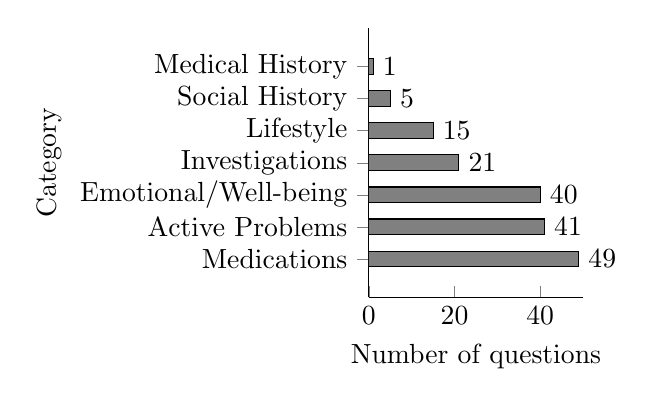
\begin{tikzpicture}
    \begin{axis}[
        xbar,
        width=4.3cm,
        height=5cm,
        bar width=0.2cm,
        nodes near coords,
        nodes near coords align={horizontal},
        xlabel={Number of questions},
        ylabel={Category},
        symbolic y coords={Medications, Active Problems, Emotional/Well-being, Investigations, Lifestyle, Social History, Medical History},
        ytick=data,
        xmin=0,
        xmax=50,
        enlarge y limits=0.2,
        axis x line*=bottom,
        axis y line*=left,
        ]
        \addplot [fill=gray, draw=black] coordinates {
            (49,Medications)
            (5,Social History)
            (41,Active Problems)
            (21,Investigations)
            (40,Emotional/Well-being)
            (15,Lifestyle)
            (1,Medical History)
        };
        % \draw[blue,dashed] ({axis cs:18.92,0}|-{rel axis cs:0,0}) -- ({axis cs:18.92,0}|-{rel axis cs:0,1}) node [pos=0.9, right] {STD = 18.92\%};
        % \draw[red,solid] ({axis cs:24.57,0}|-{rel axis cs:0,0}) -- ({axis cs:24.57,0}|-{rel axis cs:0,1}) node [pos=0.7, right] {Avg (24.57\%)};
    \end{axis}
\end{tikzpicture}
\caption{Number of questions asked in each category during the mock SRMs.}
\label{fig:question-categories}
\end{figure}

Of the four mock SMRs, a total of 117 questions were extracted from the transcripts generated by Microsoft Teams recordings. The questions were first extracted using OpenAI ChatGPT4 \cite{openai2023chatgpt4} to analyse the transcripts using this prompt "these are mock patient-doctor consultations, extract all the questions asked by the doctors". This was followed by manually checking each of the 117 questions within the video recordings to avoid transcription and extraction errors. The list of questions can be found in the first supplementary document. The questions were then grouped into these categories: conditions, medications, investigations, emotional/well-being, lifestyle, personal, and personal histories.

These categories were later presented to two of our clinician co-authors for an expert review. They made some changes in the categorisation with the final categories being \textit{active problems}, medications, investigations, emotional/well-being, lifestyle, \textit{social history} and \textit{medication history}. For the remainder of this work, we will refer to active problems as "conditions". This was followed by a review of question categorisation (which question belongs to which category on a spreadsheet) by the clinicians. The final categorisation of the questions is summarised in Figure \ref{fig:question-categories}, which shows that the highest number is 49 in the category of medications. The medical history category has the least number of questions. The top four categories by number of questions are conditions, medications, investigations, and emotional/well-being. The present work will focus on the following three categories of questions: \textbf{conditions}, \textbf{medications} and \textbf{investigations}. The number of questions in combinations of these three categories is listed in Table \ref{table:q-combination-stats}. 
\begin{table}[h]
\captionsetup{justification=justified}
\caption{The table shows the number of mock SMR questions about conditions, medications and investigations.}
\centering            % centres the whole table on the page
\begin{tabular}{>{\raggedright\arraybackslash}p{4.2cm} c}
\toprule
Combination & Question Count \\
\midrule
Medications &  35 \\
Conditions &  17 \\
Conditions, Medications &  13 \\
Conditions, Investigations &  10 \\
Investigations &  10 \\
Conditions, Medications, Investigations &   1 \\
\bottomrule
\end{tabular}
\label{table:q-combination-stats}
\end{table}

% \subsubsection{Time}
% The average time for an SMR was approximately 13 minutes (standard deviation: 4.24), and the time spent on the four main EMIS tabs is shown in Table \ref{table:smr-data-summary}. The average time spent by clinicians looking at problems, medications, investigations, and consultations was 1.65, 8.63, 3.23 and 0.47 minutes, respectively.The medication tab has the highest average, which is expected as the main aim of SMRs is a medication review. 

% ** Understanding the questions**
\subsection{Data abstraction} \label{sec:design-requirements}

\begin{table*}[ht]
\centering
\caption{The table shows breaking down questions asked during mock SMRs to generic data attributes required for each category of questions. The present work considers "dose" to be a quantitative value.}
\begin{tabularx}{\linewidth}{|X|>{\raggedright}m{2cm}|>{\raggedright\arraybackslash}m{2cm}|}
\hline
\textbf{Question} & \textbf{Data Attributes} & \textbf{Question Category} \\
\hline
What about taking the medicines because you're on quite a few. How do you feel about those?  & \multirow{3}{*}{Name} & Medications \\
Has anybody ever mentioned something called COPD to you? & & Conditions \\ 
Did he end up getting a scan in the end or not? & & Investigations \\ \hline
Have you been on the two for a long time?  & \multirow{3}{*}{Name, Date} & Medications\\ 
Have you had a recent blood test looking for hepatitis? &  & Investigations \\ 
Did that [diabetes] start later on? & & Conditions \\ \hline
I see that you're being put on some fairly strong painkillers. You don't feel very strong, no?  & Name, Dose & Medications \\ \hline
Have you ever had any specialist pain advice? & Name, Date, Severity & Conditions \\ \hline
Is that[diabetes] controlled at the moment?  & Name, Date, Quantity & Investigations \\ \hline
Here's your blood pressure?  & Quantity & Investigations \\ \hline
\end{tabularx}

\label{table:questions-to-data-attributes}
\end{table*}

Having looked at the content and duration of the SMRs, the questions were further analysed to determine the data required for each category: \textbf{conditions}, \textbf{medications} and \textbf{investigations}. The first step was to list what pieces of information are required by clinicians to answer each question within those categories (for details, see the supplemnetary material). From this list, for each of the questions, the combination of information such as name only, name and date, or a combination of name, date and other details was extracted. We call this information data attributes. For instance, for the question "Have you been on the two for a long time?" the required data was recorded as "medications" and "dates". 

The next step was to identify the data types of the information required by each question. For example, names (of conditions or medications) being "nominal". The data types used are nominal, quantitative, temporal, and ordinal. These are based on the taxonomy by Elshehaly et. al. \cite{elshehal2018taxonomy} which is based on the Vega \cite{satyanarayan2015reactive} data types. 

% There is work \cite{starren2000object} that categorises medical records into three data types: nominal, quantitative, and ordinal. 

The final step was to group the questions into possible combinations of data attributes for each category of question. The final output of this data abstraction process is summarised in Table \ref{table:questions-to-data-attributes}.

\subsection{Summary}

Four mock SMRs were performed to understand and characterise the domain problem (SMRs) believed to be the first of its kind for the purpose of a visualization design study focused on patient history visualization. The transcipts of these mock SMRs were analysed and a list of questions was extracted.  From these questions a data abstraction was generated that scoped the design study, which will be discussed next.



\input{sections/requirements}

% table should appear before the design sketches
\begin{table}[h]
\centering
% \captionsetup{justification=justified, width=\textwidth}
\captionsetup{justification=justified}
\caption{Table shows categories of data shown during SMRs, combinations of data types, and the final list of charts to generate design choices. The data types are coded as: N = Nominal, T = Temporal, Q = Quantitative and O = Ordinal}
\begin{tabular}{|m{2cm}|m{2.1cm}|m{2.2cm}|}
\hline
\textbf{Categories} & \textbf{Combinations of data types} & \textbf{Final chart options} \\
\hline
% \midrule
Investigations & Q (Quantity) & Box, Dot (Wilkinson), Histogram, Violin \\ \hline
Conditions, Medications, Investigations & N (Name) & Donut, Pie and List (Table) \\ \hline
Investigations & N, Q (Name, Quantity) & Bar, Scatter, Heatmap, Table, Pie, Donut, Radar \\ \hline
Conditions, Medications & N, T (Name, Date) & Gantt, Pie, Line, Donut, Scatter, Heatmap \\ \hline
Conditions & N, T, O (Name, Date, Severity) & Gantt, Heatmap, Line, Scatter \\ \hline
Investigations & N, T, Q (Name, Date/time, Quantity) & Gantt, Heatmap, Line, Scatter \\ \hline
\end{tabular}

\label{table:design-charts-v3}
\end{table}

\section{Visualization design}\label{sec:design}

\begin{figure}[!h]
\centering
  \begin{minipage}{0.49\textwidth}
    \includegraphics[width=\linewidth]{figures/NQ-sharp-cropped.png}
    \label{fig:figure1}
  \end{minipage}\hfill
  \begin{minipage}{0.49\textwidth}
    \includegraphics[width=\linewidth]{figures/NTO-sharp_square.png}
    \label{fig:figure2}
  \end{minipage}
    \caption{The figure shows six chart options on the top for combinations of nominal and quantitative (NQ) data and four (bottom) for combinations of nominal, temporal and ordinal (NTO) options.} 
    \label{fig:design-iterations}
\end{figure}

% design sketches (Figure 4) is moved to the mock smr section to appear at the right place

% \newcommand*\rot{\rotatebox[origin=c]{90}}
\renewcommand{\arraystretch}{1.5} 

\begin{table*}
\centering
\begin{tabularx}{\textwidth}{|p{2cm}|p{1cm}|*{7}{X|}*{3}{X|}}
\hhline{------------}
 & & \multicolumn{7}{|c|}{Magnitude channels} & \multicolumn{3}{c|}{Identity channels} \\ \cline{3-12}
Data Category & Datatype combinations & \rot{Position (?)} & \rot{Size - length (?)} & \rot{Size - area (?)} & \rot{Angle (?)} & \rot{\parbox{25mm}{Luminance (5) \\ \cite[p.223]{munzner2014visualization}}}& \rot{\parbox{25mm}{Saturation (3) \\ \cite[p.223]{munzner2014visualization}}} & \rot{\parbox{25mm}{Transparency (2) \\ \cite[p.225]{munzner2014visualization}}} & \rot{\parbox{25mm}{Hue (7) \\ \cite[p.224]{munzner2014visualization}}} & \rot{\parbox{25mm}{Texture (24) \\ \cite[p.240]{munzner2014visualization}}} & \rot{\parbox{25mm}{Shape (24) \\ \cite[p.238]{munzner2014visualization}}} \\ \hline
Con. Med. Inv. & N & &  &  &  &  & & & N &N &N \\ \hline
Inv. & Q &Q & Q & Q & Q &Q? & Q? & Q? &  & & \\ \hline
Con. Med. & N,T & & T & T & T &  & & & N &N &N \\ \hline
Inv. & N,Q &Q & Q & Q & Q &Q? & Q? & Q? & N &N &N \\ \hline
Con. & N,T,O & &TO &TO &TO & O &O &O & N &N &N \\ \hline
Inv. & N,Q,T &Q &QT &QT &QT & Q?T & Q? & Q? & N &N &N \\ \hline
\end{tabularx}
\caption{The table shows categories of questions grouped by their data attributes in the first two columns, mapped to possible representation channels and channel limitations within visualization guidelines. The number next to channel name is the reported limit while the question mark indicates lack or no limit. Data types are encoded as: N = Nominal, Q = Quantitative, T = Temporal and O = Ordinal.}
\label{table:channels-guidelines}
\end{table*}


In this section, the approach and results of generating design choices for the domain problem (clinicians conducting SMRs) are described. Generating these choices involved a two-step process: exploring the design space for design choices and evaluating them.

\subsection{Design space exploration} \label{sec:design-explore-space}

The exploration of the design space based on charts was carried out according to the design guidelines and principles within the visualization literature. In this step of the design study, how each of the chart design choices would be limited by guidelines such as those of Munzner \cite{munzner2014visualization} and Spence \cite{spence2001information} was checked. Specifically, visual encoding channels such as position, size, shape, etc. The context of magnitude (quantitative values) and identity (nominal values) of each chart option were checked and noted. For example, in the case of identity channels such as colour hue, a limit of seven bins is recommended \cite{munzner2014visualization}.

% **could add a diagrame**

To generate chart design options for each of the combinations of data types, a comprehensive list of charts was prepared from the charts appearing Tables \ref{table:dashboards} and \ref{table:ehr-star} as well as Data Visualization Survey's 2021 chart lists \cite{dvssurvey2021}. For each chart option in the list, the possible channel was recorded to encode each of the data type combinations (see Section \ref{sec:design-requirements}). For instance, the height of a bar chart could be used to encode quantitative as well as temporal data types. We then filtered the charts based on the matching data types of the data type combinations for the three categories of SMR data: conditions, medications and investigations.

The final list of chart options for each of the categories of mock SMR questions is listed in Table \ref{table:design-charts-v3}. Each chart choice in this table appears in the two review publications (Dowding et al. \cite{dowding2015dashboards} and Wang and Larame \cite{wang2022ehr}) or the original publications cited by them.

This step was followed by three rounds of pencil and paper sketches excluding the fourth round of finalising the design options for evaluation over several weeks. In each iteration, the focus was only on a combination of data types such as "NQ" (nominal, quantitative), and which category of questions the data would be visualized under (e.g. conditions). A pencil and paper sketching is more flexible and provides unrestricted space \cite{hakkarienn2000} for being creative without restrictions compared to writing code from the beginning. Figure \ref{fig:design-iterations} shows two sets of design choices for the two combinations of data types: nominal, quantitative (N, Q) and nominal, temporal and ordinal (N, T, O). These two sets are two of the six data combinations shown in Table \ref{table:design-charts-v3} (second column). 

For each combination of data types, similar visualization channel encoding, such as the use of area for the same data type using different chart type, was avoided. This also enabled us to discard "similar" design options (chart types) from the initial large list of options. For example, in the design choices for nominal, temporal and ordinal (N, T, O) data types in Figure \ref{fig:design-iterations} (right), a bar chart would be too similar to a Gantt chart and that is why the bar chart does not appear as a design choice, as Gantt charts were deemed to be more appropriate.

% The next step was to evaluate these chart options which will be discussed next.

% \begin{figure}[ht]
%   \centering
%   \includegraphics[width=8cm]{figures/design-process.png}
%   \caption{Figure caption here.}
%   \label{fig:design-process}
% \end{figure}

% now in teaser
% \begin{figure*}[!h]
% \centering
%   \begin{minipage}{\textwidth}
%     \includegraphics[width=\linewidth]{figures/indiv-results.png}
%     \label{fig:indvid-results}
%   \end{minipage}
%     \caption{The individual results of all of the charts design choice evaluation. Each stacked bar chart is marked with the question number within the evaluation and the category of data types for which the design choices were shown to the participants.} 
%     \label{fig:indvidual-results}
% \end{figure*}

\subsection{Design choice evaluation}
% The next step of the design space exploration process was to evaluate the chart choices.

% \begin{figure}[ht]
%   \centering
%   \includegraphics[width=7cm]{figures/q4-n.png}
%   \caption{The figure shows three design choices for the category of nominal data type. The design choices are all drawn within the same spaces on A4 sheets before being scanned. }
%   \label{fig:q4-n}
% \end{figure}

\subsubsection{Method}
The participants for the evaluation were chosen to be both domain experts (co-authors) and members of the research project team. All of the team were invited to participate and 18 responded.

In terms of materials, the final designs were generated for the list of charts for each of the combinations listed in Table \ref{table:design-charts-v3}. These were drawn within equal-sized on A4 sheets and scanned. Each chart was populated with three rows of data. The same quantitative values were repeated to create a list of 10 in the case of box, dot and violin charts for the quantitative data type. This was deemed a minimal data set to assess the effectiveness of each chart and the assumption that a chart failing at this minimal level would likely be unsuitable for a larger quantity of data.

The procedure for evaluating the design choices involved presenting the charts to participants using Microsoft Forms. The form contained two questions about the participant's self-identified "profession" and "years in the current profession". There were also six questions; one for each combination of data types in Table \ref{table:design-charts-v3}. Each of these questions included an image with the design choices for the combination of data such as those in Figure \ref{fig:design-iterations}. For each of the six questions, the participants were asked this question: "To what extent do you agree with the statement: 'The chart effectively communicates the information it contains'?". There was also this instruction to answer the question "Select 'Agree' if you think the charts effectively communicate the data, 'Neutral' if you are uncertain or find some charts more effective than others, and 'Disagree' if you think the chart fails to communicate the data effectively." The responses were collected using Microsoft Forms for analysis which will be discussed next.

\subsubsection{Results}

A total of 18 participants returned the questionnaire. 
Individual results for each of the six combinations of data types showed clear winners, such as histograms having no "disagree" answers when looking at quantitative data, and likewise, the Gantt chart having no "disagree" answers in the category of nominal and temporal data types as shown in Figure \ref{fig:indvidual-results}. Notably, violin plots received few (3 out of 18) "agree" answers in the quantitative data combination, and donut (doughnut) chart had no "agree" answers in the nominal and temporal data type combination.

\begin{figure*}[ht]
  \centering
  \includegraphics[width=\textwidth]{figures/indiv-results.png}
  \caption{The individual results of the charts design choice evaluation. Each chart is labelled with the question number within the questionnaire and the category of data types for which the design choices were shown to the participants.}
  \label{fig:indvidual-results}
\end{figure*}

Looking at each question and starting with question three in Figure \ref{fig:indvidual-results}, the histogram had the highest "agree" responses given the small data set used in the study. In question four, when looking at the choices for showing a list of names (nominal only), the difference between "agree" answers for "List (Table" and a pie chart is small (66\% versus 61\%). Question five included the design choices for nominal and quantitative data using seven different chart types. Bar charts had the highest "agree" answers. Question six was showing nominal and temporal data, only Gantt and line charts had no "disagree" answers, while donut chart was the only choice with no "agree" answers. Question seven included four design choices for nominal, temporal and ordinal data, only scatter plots received less than 50\% "agree" answers. Question eight used the same four choices from question seven to visualise nominal, temporal and quantitative data. All but Gantt charts received less than 50\% "agree" responses.


\subsubsection{Discussion}
The evaluation aimed to find which charts were effective for representing the simple data set, providing a shortlist of design choices for further investigation.
A starting point was to include each chart where at least 50\% of participants agreed that the chart was effective for a given combination of data types.
However, there were exceptions.

The shortlist for quantitative data comprised a histogram, box plot and dot plot. However, box plots only show unimodal distributions and histograms may hide sophistcated data distributions when the default number of bins (e.g., 10) is used.
By contrast, violin plots are designed for multimodal distributions and those often occur in health data~\cite{ruddle2024tasks}.
It is also worth noting that pie and donut charts are essentially the same as each other, except that a donut has a hole in the middle.
However, donut charts are less common so people are less famiiar with them, which explains why fewer participants agreed that a donut would be effective for the data type combinations where donut and pie charts were investigated. 

The final shortlist contained the following:
\begin{itemize}
  \item Quantitative: Histogram, box, dot and violin
  \item Nominal: List (Table) and pie
  \item Nominal and quantitative: Bar, table and scatter
  \item Nominal and temporal: Gantt chart and line
  \item Nominal, temporal and ordinal: Gantt chart, line and heatmap
  \item Nominal, temporal and quantitative: Gantt chart
\end{itemize}


\section{Conclusions and future work} \label{sec:conclusions}
% The aim of the visualization work package within the DynAIRx project is to generate visual summaries to assist clinicians with medicine optimisation (SMRs are an opportunity to do so). 
The present work started with reviewing techniques to visualise EHR. Using four mock SMRs the domain problem was characterised and data abstraction was generated to carry out the chart-type design space exploration described in the previous sections. Through exploration of the design space, a list of charts was selected and evaluated. The designs were then implemented in a Python package to generate the same visualizations using 2.1M real patient data from the CPRD. We anticipate that the Python package can be usable for other datasets similar to the CPRD data types used in this study.

The contributions of the present work are based on the three main contributions outlined in the method paper by Sedlmair, Meyer, and Munzner \cite{sedlmair2012design}: problem characterisation, that is, analysis and data abstraction using mock SMRs, the design study to present candidate chart types and a Python package-based implementation. 

% The design study approach of the present work is believed to be reproducible and could be applied to other domain problems.

The present work enables us and other visualization designers looking at generating "integrated" dashboards to use the chart types in this study and the Python package implementation to visualise complete patient records to assist clinicians conducting medication review such as SMRs.

\section*{Acknowledgements}
None

%-------------------------------------------------------------------------
% \newpage
%\bibliographystyle{eg-alpha}
\bibliographystyle{eg-alpha-doi}

\bibliography{bibdynairx}

%-------------------------------------------------------------------------
\end{document}
